\section{Results}
\label{sec:stop_results}

% unblinded plots
% yields
% exclusion contour
%   -> standalone 3-body
%   -> SUSY summary plot with 36/fb result

A profile likelihood fit is performed, including all of the CRs and SRs of the analysis.
In order to assess the compatibility of the observed data in the SRs with the predicted
SM background, the observed data in the SRs is also provided in the fit as a constraint.
The result of running this fit, with the added SRs and the observed data therein,
is shown in Table~\ref{tab:stop_srs_postfit}.
Even though we have added the additional data constraint from the SRs, the post-fit normalisation
correction factors derived for the \ttbar~and diboson processes are consistent
with those derived in the background-only fit configuration described in Section~\ref{sec:stop_background_only},
due to the larger statistical power of the data counts observed in the CRs, as opposed to the low numbers
observed in the SRs.

It can be seen in Table~\ref{tab:stop_srs_postfit} that there is no significant deviation
between the observed data counts in the SRs as compared to the post-fit prediction of the total SM
background.
The largest null-hypothesis $p_0$-value in these regions, giving the incompatibility of the observed
data with the predicted SM background, is associated with the region SRt-SF and is $p_0 = 0.15$, still
quite far from the $p_0 = 0.05$ critical value.
Figure~\ref{fig:stop_sr_unblinded} shows a few kinematic distributions in the SRs with the post-fit
MC prediction compared to the observed data.
In these plots, the SR selection on the variable being plotted has been removed.

As there is no significant deviation between the prediction and observed data, hypothesis tests are performed in order to assess which regions
of the \bWN parameter space can be excluded.
As described in Section~\ref{sec:stat_hypo}, we use the \cls construction to determine whether
a given point in the \msn plane is excluded at 95\% CL.
Hypothesis tests are run over the \bWN signal grid, with all four SRs and three CRs included in the profile
likelihood along with the observed data in all regions included.
The results of the hypothesis tests are illustrated in Figure~\ref{fig:stop_limplot}, showing the
exclusion regions in the \bWN region of the \msn plane.

\begin{table}[!htb]
    \begin{center}
        \caption{
            Observed and predicted yields in the SRs for the \bWN search.
        }
        \label{tab:stop_srs_postfit}
        \begin{tabular}{l| c c c c}
            \hline
            \hline
                & \multicolumn{4}{c}{\textbf{Regions}} \\
            \hline
            \textbf{Process} & \textbf{SRw-SF} & \textbf{SRw-DF} & \textbf{SRt-SF} & \textbf{SRt-DF} \\
            \hline
            Observed Data & 4 & 6 & 6 & 6 \\
            \hline
            Post-fit Total SM & $9.83 \pm 3.57$ & $7.84 \pm 3.09$       & $3.10 \pm 1.42$ & $4.40 \pm 1.87$ \\
            \hline
            Post-fit \ttbar & $4.18 \pm 1.65$ & $4.57 \pm 2.18$         & $2.54 \pm 1.34$ & $3.58 \pm 1.77$ \\
            Post-fit Diboson & $3.43 \pm 2.27$ & $2.88 \pm 1.44$        & $0.16 \pm 0.09$ & $0.04 \pm 0.03$ \\
            \hline
            SM & $9.52 \pm 3.41$ & $7.53 \pm 2.84$                      & $2.95 \pm 1.34$ & $4.20 \pm 1.77$ \\
            \hline
            \ttbar & $3.95 \pm 1.55$ & $4.31 \pm 2.06$                  & $2.40 \pm 1.28$ & $3.38 \pm 1.68$ \\
            Diboson & $3.35 \pm 1.58$ & $2.82 \pm 1.22$                 & $0.16 \pm 0.06$ & $0.04 \pm 0.03$ \\
            Single-top & $0.31 \pm 0.29$ & $0.23 \pm 0.12$              & $0.12 \pm 0.05$ & $0.14 \pm 0.08$ \\
            $Z$+jets & $1.47 \pm 1.47$ & $0.05 \pm 0.01$                & $0.10 \pm 0.03$ & $0.00 \pm 0.00$ \\
            $\ttbar + V$ & $0.03 \pm 0.01$ & $0.06 \pm 0.02$            & $0.18 \pm 0.05$ & $0.24 \pm 0.07$ \\
            Fakes & $0.42 \pm 0.28$ & $0.06 \pm 0.06$                   & $0.00 \pm 0.00$ & $0.41 \pm 0.09$ \\
            \hline
            \hline
        \end{tabular}
    \end{center}
\end{table}

\begin{figure}[!htb]
    \begin{center}
        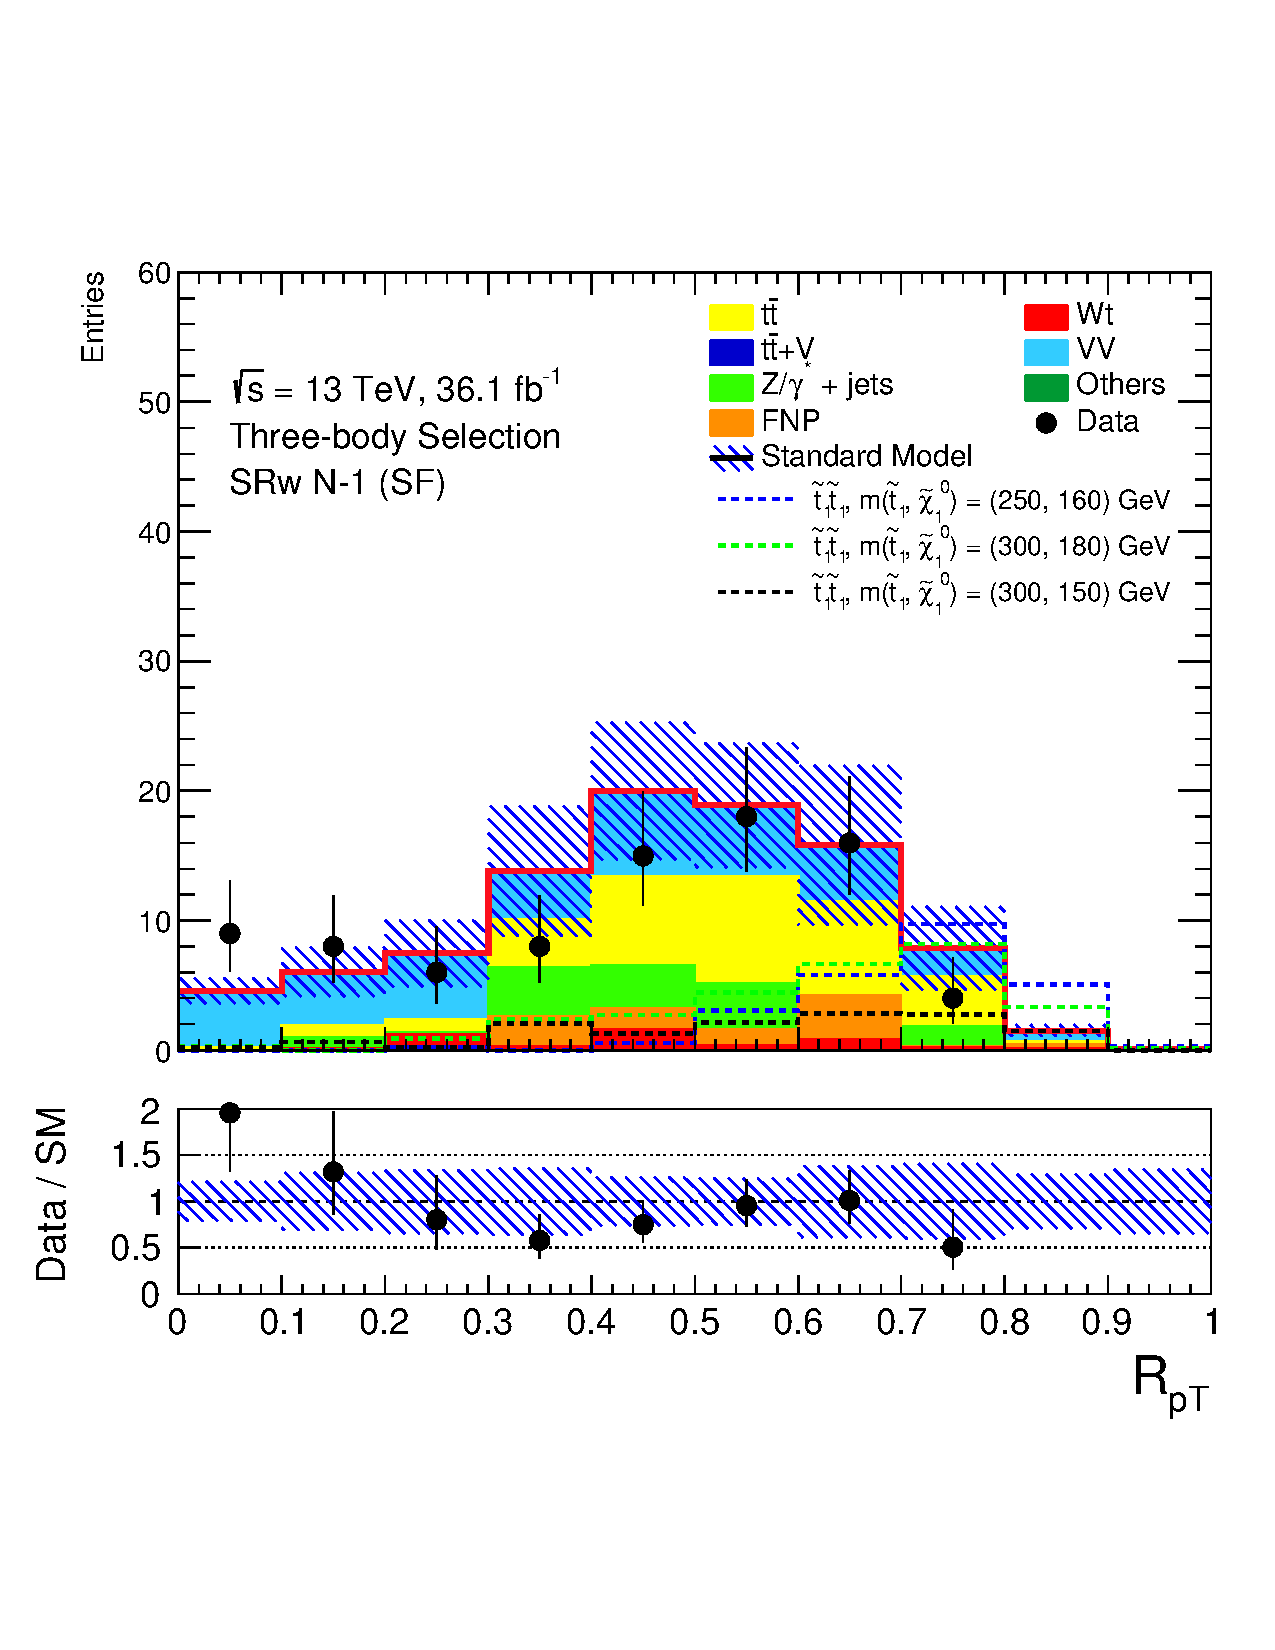
\includegraphics[width=0.48\textwidth]{figures/search_stop2l/results/srwNM1SF_RPT_nm1}
        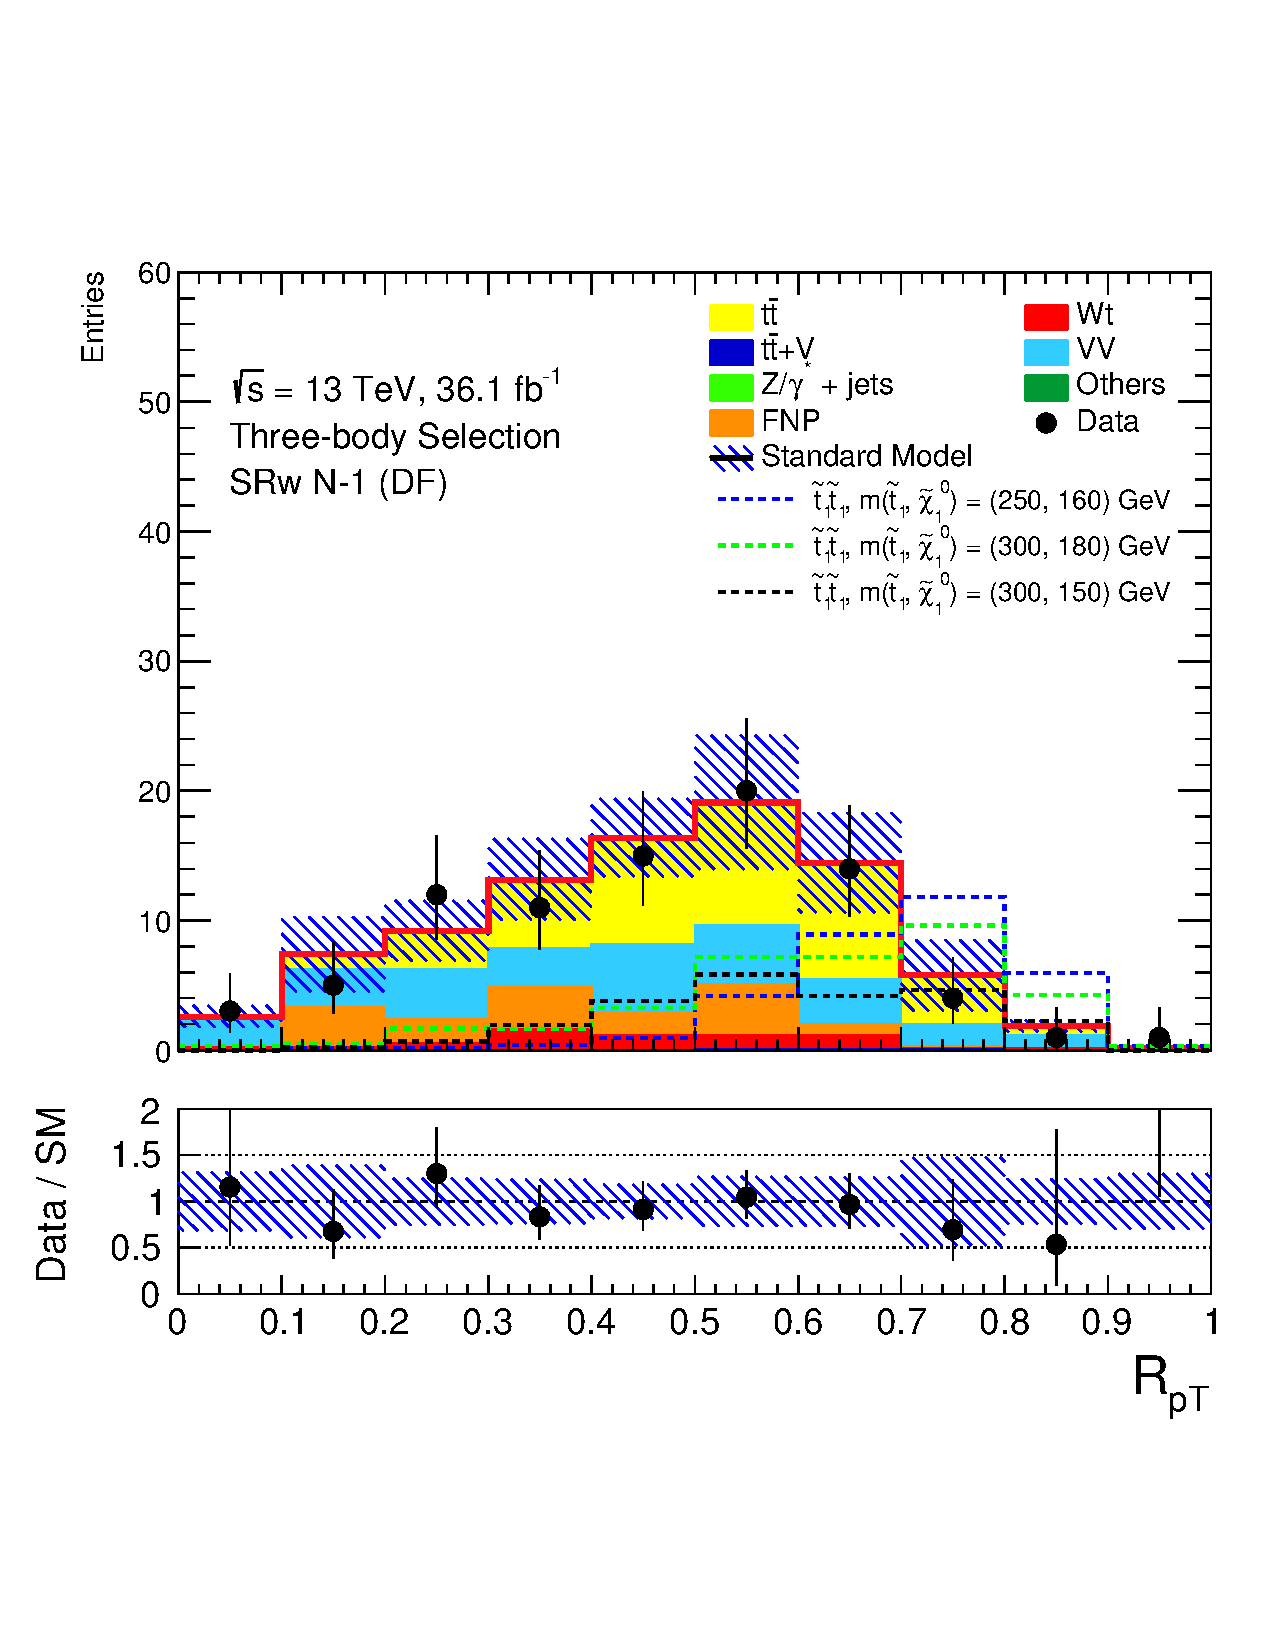
\includegraphics[width=0.48\textwidth]{figures/search_stop2l/results/srwNM1_RPT_nm1}
        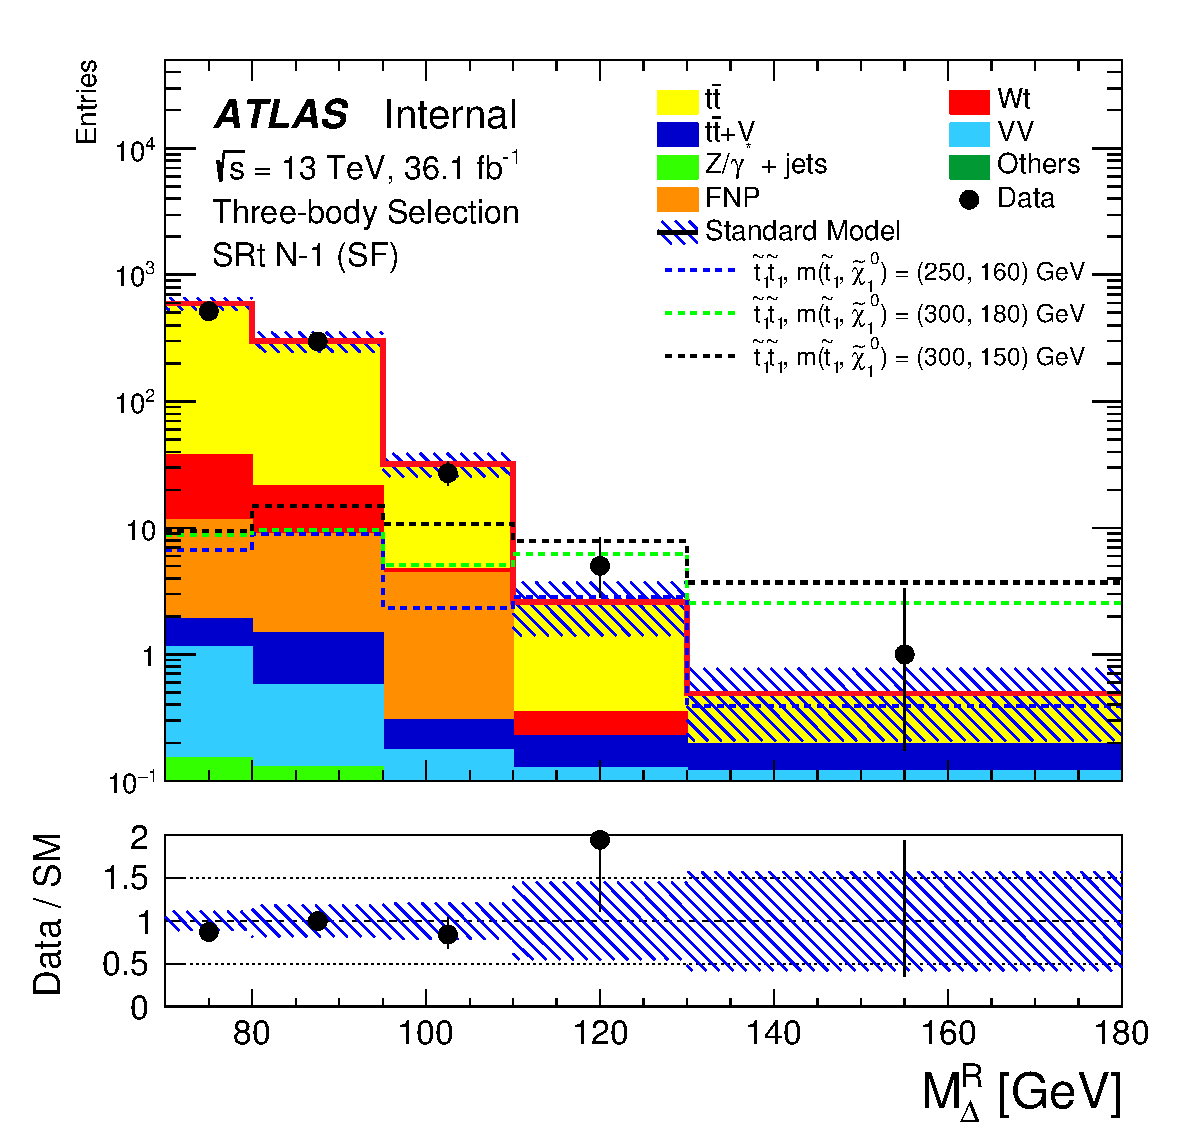
\includegraphics[width=0.48\textwidth]{figures/search_stop2l/results/srtNM1SF_MDR_nm1}
        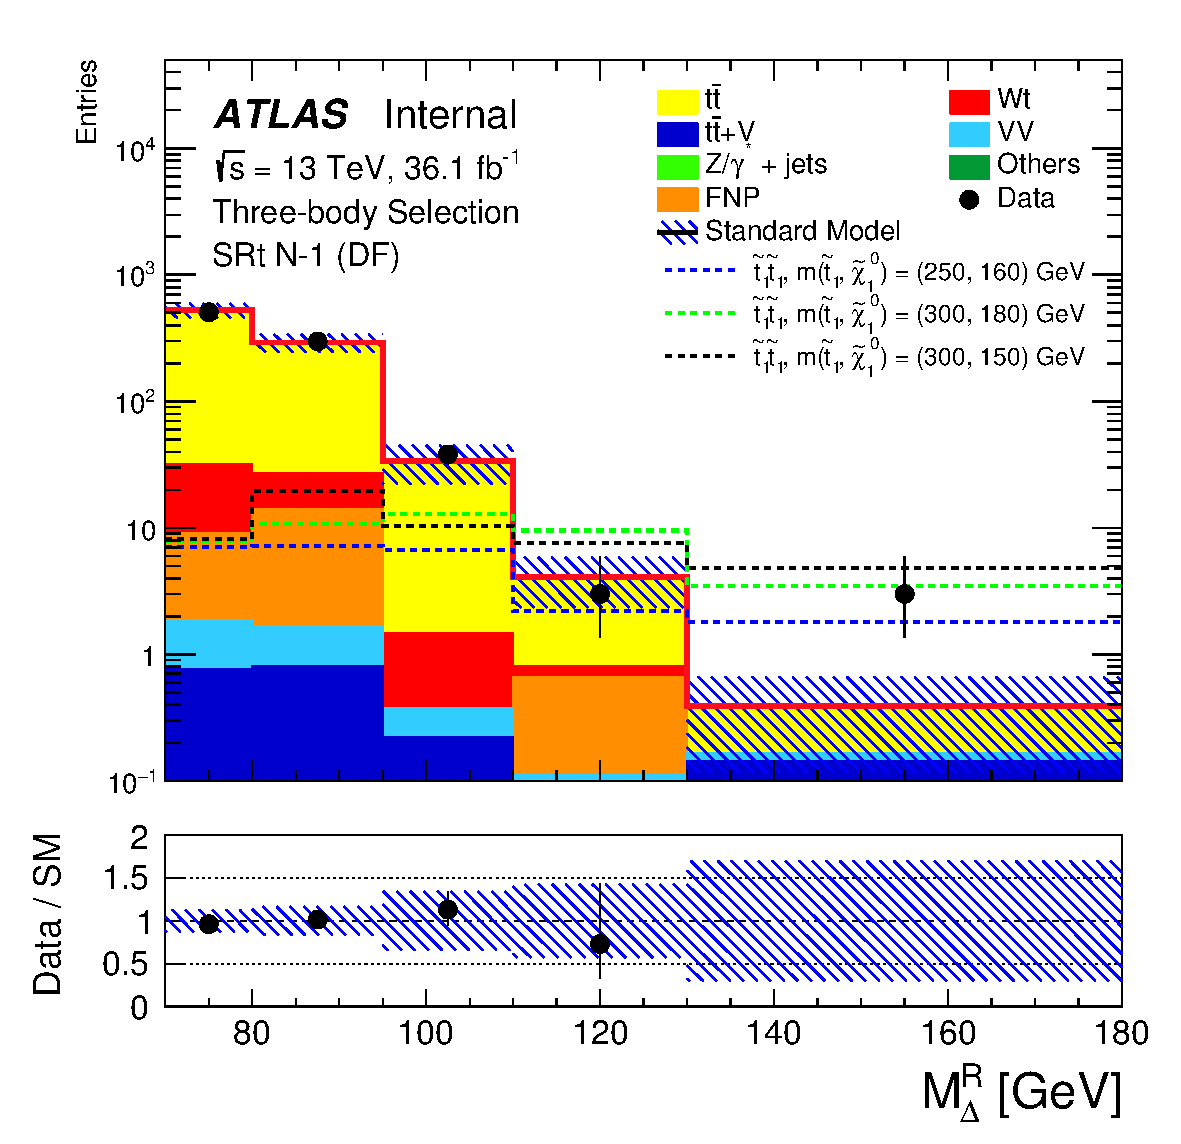
\includegraphics[width=0.48\textwidth]{figures/search_stop2l/results/srtNM1_MDR_nm1}
        \caption{
            \textit{\textbf{Top}}: Distributions of \rpt in SRw-SF (\textit{left}) and SRw-DF (\textit{right}), with the observed data.
            \textit{\textbf{Bottom}}: Distributions of \mdr in SRt-SF (\textit{left}) and SRt-DF (\textit{right}), with the observed data.
            The selection on the variable being plotted, in the corresponding SR, has been removed from the selection applied
            to the events populating the histogram bins.
            The hatched bands indicate the statistical and systematic uncertainty on the background estimate.
            The dashed lines show the MC simulated signal processes for the three benchmark \bWN signal samples
            at $\msn = (250,160)$, $(350,180)$, and $(350,150)$\,GeV.
        }
        \label{fig:stop_sr_unblinded}
    \end{center}
\end{figure}

\begin{figure}[!htb]
    \begin{center}
        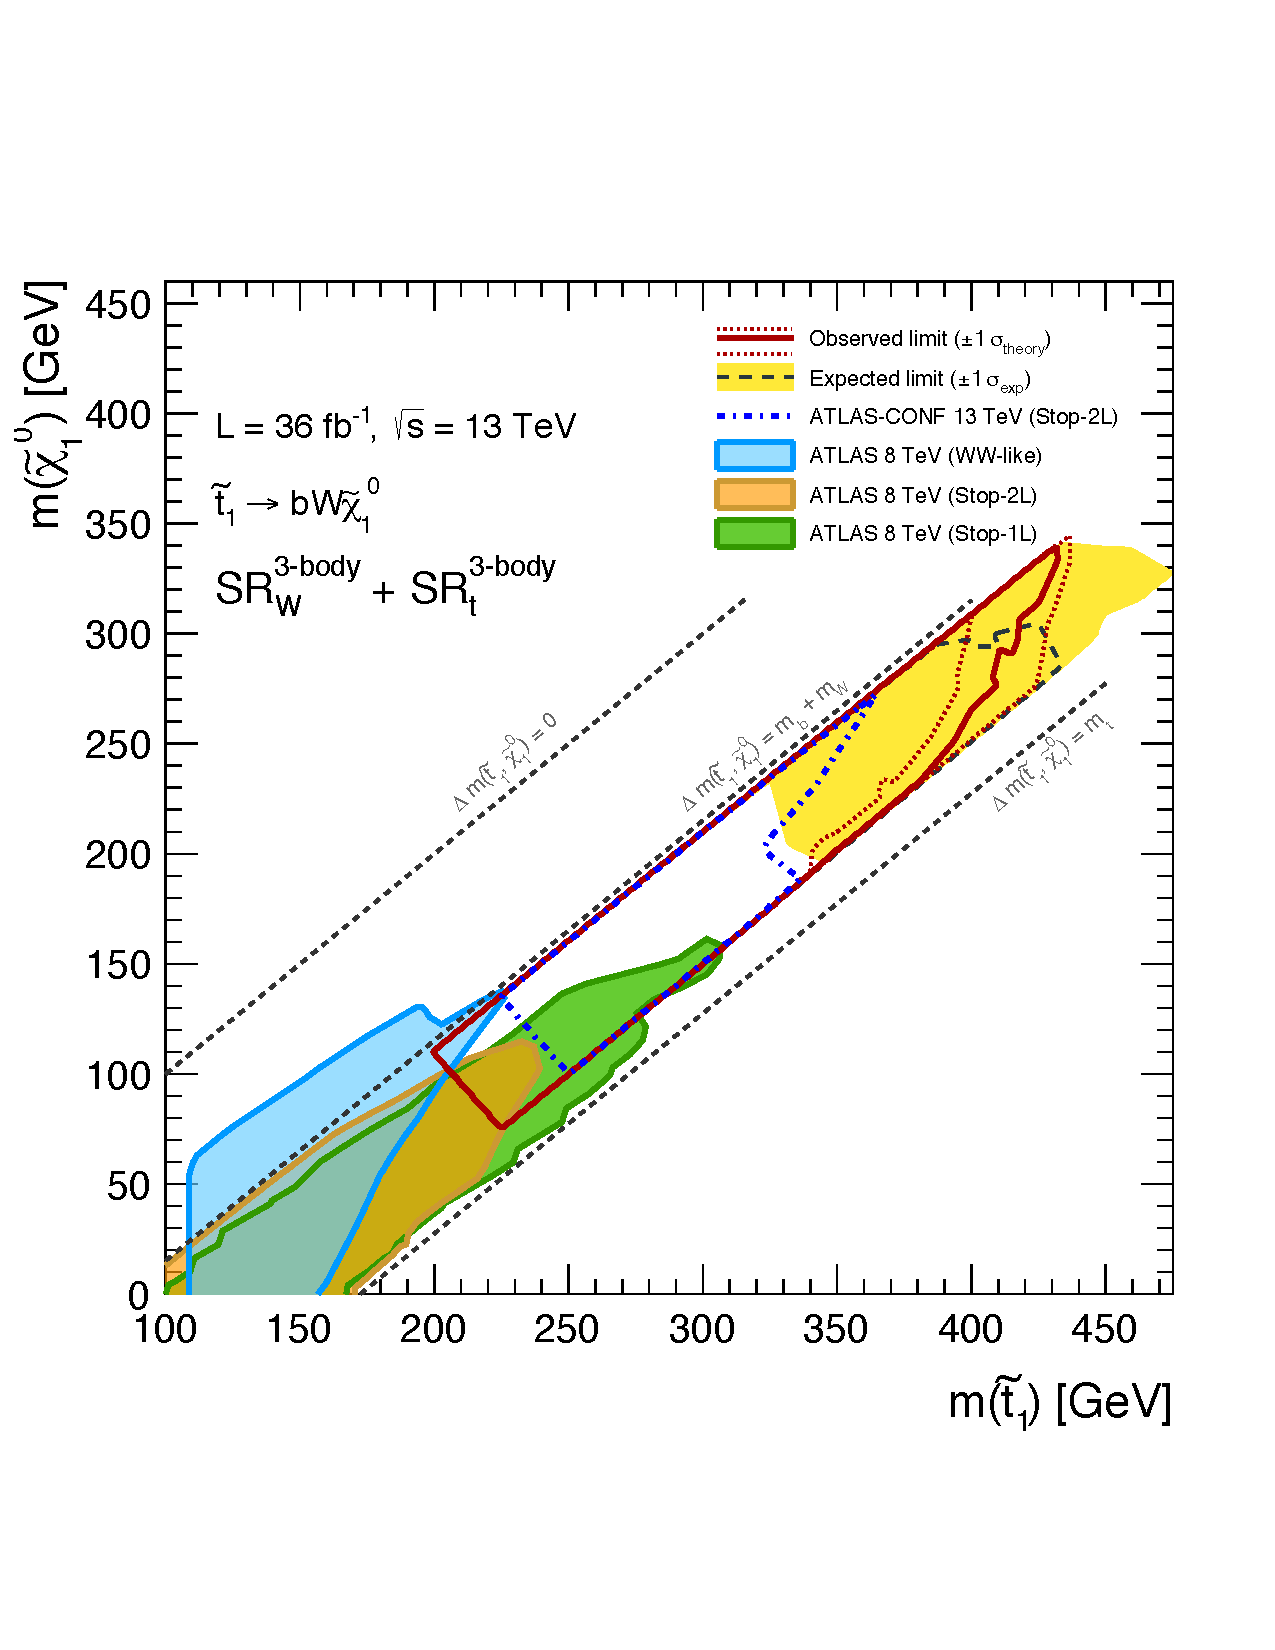
\includegraphics[width=0.7\textwidth]{figures/search_stop2l/results/limplot_SRwt_bWN_sfdf}
        \caption{
            95\% CL exclusion contours for the 2015+2016 search for the \bWN process.
            Shown for comparison are the Run 1 8 TeV results for the same
            \bWN scenario, both in the one (`Stop 1L') and two (`Stop 2L' and `WW-like') lepton channels.
            The $\pm1 \sigma_{\text{theory}}$ lines on the observed limits correspond to varying the \bWN signal
            predicted cross-section values up and down within their theoretical uncertainty and re-running the 
            hypothesis tests.
            The dashed blue exclusion contour is a previous iteration of the current analysis, but
            based on a reduced dataset ($3.2$\,fb$^{-1}$, based only on data collected in 2015, as opposed to $36$\,fb$^{-1}$) and is shown also for comparison purposes.
        }
        \label{fig:stop_limplot}
    \end{center}
\end{figure}
